% This file contains the header data for all assignment files
\documentclass[onecolumn, 11pt]{article}

\usepackage{bbold}   %Get fancy double struck math notation for sets
\usepackage{cite}
\usepackage{cleveref}
\usepackage{color}
\usepackage{courier}   %Have code written out nicely
\usepackage{float}
\usepackage[top=1in, bottom=1in, left=1in, right=1in]{geometry}
\usepackage{graphicx} % handles graphics and figures
\usepackage{hyperref}
\usepackage{listings}
\usepackage{mathtools,bm}
\usepackage{multicol}

\catcode`\^^M=10      %  Makes blank lines meaningless, force use of \par

\definecolor{magenta}{rgb}{0.8,0.0,1.0}
\definecolor{darkGreen}{rgb}{0.0,0.4,0.0}
\definecolor{blue}{rgb}{0.0, 0.0, 0.9}
\definecolor{purple}{rgb}{0.7, 0.0, 0.7}
\definecolor{darkGreen}{rgb}{0.0,0.4,0.0}

\newcommand{\quotes}[1]{``#1''}
\newcommand{\todo}[1]{{\color{magenta}\par {[{\bf ToDo: } {\em #1}} ] \\    }}

\newcommand{\norm}[1]{\left\lVert#1\right\rVert}

%%%%%%%%%%%%%%%%%%%%%%%%%%%%%%%%%%%%%%%%%%%%%%%%%%%%%%%%%%%%%%%%%%%%%%%%%%%%%%%
% NOTE:
%
% The following block of commands is used to format Matlab code blocks for the
% listings package. This block of code is based on two examples:
%  -->   https://gist.github.com/eyliu/120689
%  -->   http://links.tedpavlic.com/ascii/homework_new_tex.ascii
%
% Import file block using:
%   \lstinputlisting{fileName.m}
%
\lstloadlanguages{Matlab}
%
\lstset{language=Matlab,                        % Use MATLAB
        frame=single,                           % Single frame around code
        basicstyle=\small\ttfamily,             % Use small true type font
        keywordstyle=[1]\color{blue}\bfseries,  % MATLAB functions bold and blue
        keywordstyle=[2]\color{purple},         % MATLAB function arguments purple
        keywordstyle=[3]\color{blue}\underbar,  % User functions underlined and blue
        identifierstyle=,                       % Nothing special about identifiers
                                                % Comments small dark green courier
        commentstyle=\usefont{T1}{pcr}{m}{sl}\color{darkGreen}\small,
        stringstyle=\color{darkGreen},            % Strings are purple
        showstringspaces=false,                 % Don't put marks in string spaces
        tabsize=4,                              % 4 spaces per tab
        %
        %%% Put standard MATLAB functions not included in the default
        %%% language here
        morekeywords={xlim,ylim,var,alpha,factorial,poissrnd,normpdf,normcdf},
        %
        %%% Put MATLAB function parameters here
        morekeywords=[2]{on, off, interp},
        %
        %%% Put user defined functions here
        morekeywords=[3]{FindESS, homework_example},
        %
        morecomment=[l][\color{blue}]{...},     % Line continuation (...) like blue comment
        numbers=left,                           % Line numbers on left
        firstnumber=1,                          % Line numbers start with line 1
        numberstyle=\tiny\color{blue},          % Line numbers are blue
        stepnumber=5                            % Line numbers go in steps of 5
        }
%
%%%%%%%%%%%%%%%%%%%%%%%%%%%%%%%%%%%%%%%%%%%%%%%%%%%%%%%%%%%%%%%%%%%%%%%%%%%%%%%


% Special settings for matlab code on exam
\lstset{morekeywords={runSloppySimulation,runSimBadly,simStepMidpointMethod}}

\newcommand{\scoreMark}[0]{$\rule{1.5cm}{0.15mm}$ / $\rule{1.5cm}{0.15mm}$}

%========================================================================
\title{ME 149:  Midterm Exam}
\date{March 15  ---  Start: 6:00pm  ---  End: 7:15pm}
\author{Optimal Control for Robotics}
%========================================================================
\begin{document}
\maketitle

\begin{abstract*}
No calculators, notes, books, or computers allowed. Total time:  75 minutes.
\end{abstract*}
%=================================================

\vspace{1em}

\section*{Student Name:  $\rule{10cm}{0.3mm}$}

\vspace{1em}

\section*{How to optimize your score?}

\begin{itemize}  \setlength\itemsep{0.1em} \setlength\itemindent{18pt}
  \item Be neat and well organized
  \item For longer problems, show intermediate steps and box your
  \fbox { \parbox{3em}{answer} }
  \item If you need extra space...
        use the back of the page,
        the final (blank) page of the exam,
        or ask for more paper.
        Clearly indicate where the extra work is.
  \item Define all variables that you use and state any assumptions that you make.
\end{itemize}


\vspace{1em}

\section*{Score:  \scoreMark}
\vspace{1em}
\begin{large}
\begin{multicols}{2}
\begin{enumerate}  \setlength\itemsep{1.1em} \setlength\itemindent{36pt}
\item \scoreMark
\item \scoreMark
\item \scoreMark
\item \scoreMark
\item \scoreMark
\item \scoreMark
\item \scoreMark
\item \scoreMark
\item \scoreMark
\end{enumerate}
\end{multicols}
\end{large}


% Force enumerated lists to use letters
\renewcommand{\theenumi}{\Alph{enumi}}

%~~~~~~~~~~~~~~~~~~~~~~~~~~~~~~~~~~~~~~~~~~~~~~~~~~~~~~~~~~~~~~~~~~~~~~~~~~~~~

\pagebreak
\section{Newton's Method}

\begin{enumerate}
  \item Suppose that you want to solve the scalar nonlinear equation $f(x) = 0$. \\
        The current estimate of the root is given by $x_k$
        and the next estimate of the root is given by $x_{k+1}$.
        Derive the Newton-Rhapson update that computes $x_{k+1}$ given $x_k$.
  \vspace{25em}
  \item What is the difference between the Newton--Rhapson
        and the secant methods for scalar root finding?
        In what situation would you prefer one to the other?

  \pagebreak
  \item Draw a figure that clearly demonstrates a situation in which
        Newton's method will fail to converge to a root of the function.
        Why does the Newton--Rhapson method fail in this situation?
  \vspace{25em}
\end{enumerate}


%~~~~~~~~~~~~~~~~~~~~~~~~~~~~~~~~~~~~~~~~~~~~~~~~~~~~~~~~~~~~~~~~~~~~~~~~~~~~~

\section{Midpoint Method Implementation}

Implement the function \texttt{simStepMidpoint()} on the following page.
This function computes a single simulation step using the midpoint method.
You code should be clear, correct, and follow the best practices that
have been discussed throughout the course.
Use the space below for planning your solution.
Write your Matlab code inside of the function template on the following page.



\pagebreak
\lstset{stepnumber=0}
\lstinputlisting{simStepMidpoint.m}



\pagebreak
\section{Bisection Search}
\begin{NoHyper}
Use a bisection search to iteratively reduce the interval that is known
to bracket the root of the function shown in Figure \ref{fig:RootSolveExampleFigure}.
\textbf{Populate the table below}, showing the bracket for the first five iterations
and the new point that will be evaluated on that iteration.
\end{NoHyper}
\begin{itemize}  \setlength\itemsep{0.3em}
  \item \texttt{Iter 0:   bracket: [-1.000,  \hspace{2.9em} 1.000]  \hspace{1em}  xNew = }
  \item \texttt{Iter 1:   bracket: [ \hspace{10em} ]  \hspace{1em}  xNew = }
  \item \texttt{Iter 2:   bracket: [ \hspace{10em} ]  \hspace{1em}  xNew = }
  \item \texttt{Iter 3:   bracket: [ \hspace{10em} ]  \hspace{1em}  xNew = }
  \item \texttt{Iter 4:   bracket: [ \hspace{10em} ]  \hspace{1em}  xNew = }
\end{itemize}

\begin{figure}[ht]
	\centering
  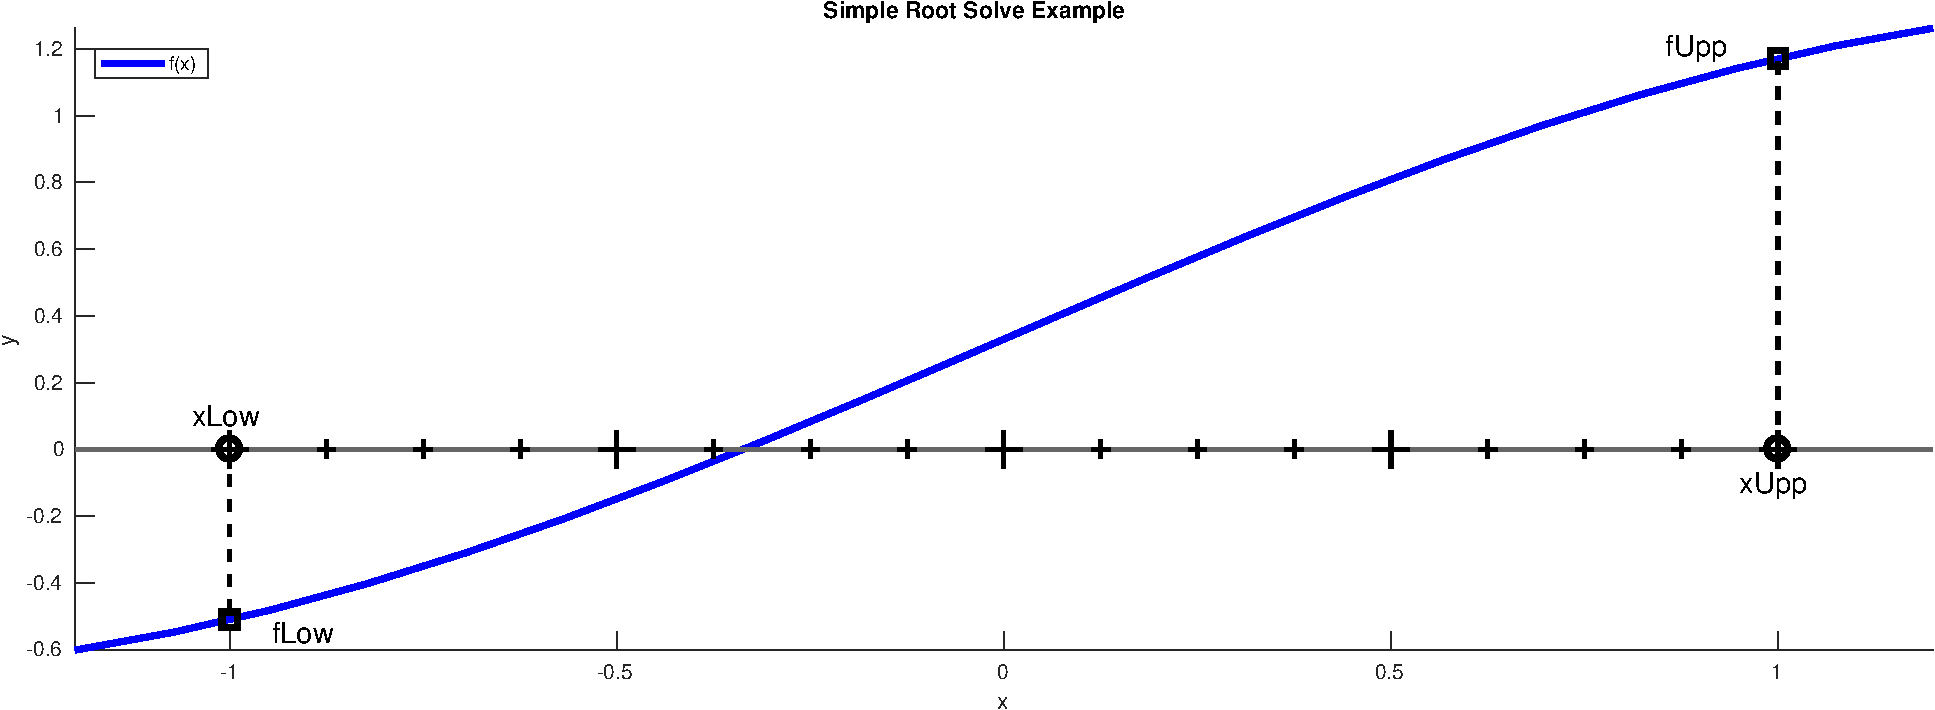
\includegraphics[width=\textwidth]{RootSolveExampleFigure.pdf}
  \caption{Bisection Search Example Figure}
  \label{fig:RootSolveExampleFigure}
\end{figure}



%~~~~~~~~~~~~~~~~~~~~~~~~~~~~~~~~~~~~~~~~~~~~~~~~~~~~~~~~~~~~~~~~~~~~~~~~~~~~~

\pagebreak
\section{Scalar Taylor Series}

Write Taylor series approximation of $f(t)$ to second-order around the point $t_0$.

\vspace{2em}
\begin{equation*}
  f(t) \approx \hspace{50em}
\end{equation*}
\vspace{7em}

\section{Vector Taylor Series}

Write the Taylor series approximation of $f(t, \bm{x}, \bm{u})$ to first-order
about the point: $t_0$, $\bm{x}_0$, and $\bm{u}_0$.

\vspace{2em}
\begin{equation*}
  f(t, \bm{x}, \bm{u}) \approx \hspace{46em}
\end{equation*}
\vspace{4em}

%~~~~~~~~~~~~~~~~~~~~~~~~~~~~~~~~~~~~~~~~~~~~~~~~~~~~~~~~~~~~~~~~~~~~~~~~~~~~~

\pagebreak
\section{Function Handle Gymnastics}
\textbf{What will the following script print to the command prompt?} \\
For each part A, B, C, show your work and then put a box around
the text that Matlab will print to the command prompt.

\lstinputlisting{functionHandleGymnastics.m}

\subsection*{Part A:}
\vspace{7em}
\subsection*{Part B:}
\vspace{9em}
\subsection*{Part C: }
\vspace{11em}


%~~~~~~~~~~~~~~~~~~~~~~~~~~~~~~~~~~~~~~~~~~~~~~~~~~~~~~~~~~~~~~~~~~~~~~~~~~~~~

\pagebreak
\section{Matlab Programming Style}
The program below simulates a simple pendulum. It works, but is written poorly. \\
\textbf{Clearly identify at least 5 distinct issues with the code.}

\lstset{stepnumber=1}
\lstinputlisting{runSloppySimulation.m}

\vspace{30em}


%~~~~~~~~~~~~~~~~~~~~~~~~~~~~~~~~~~~~~~~~~~~~~~~~~~~~~~~~~~~~~~~~~~~~~~~~~~~~~


\pagebreak
\section{Linearized Dynamical System}

Given the non-linear system dynamics described below,

\begin{equation*}

  \dot{\bm{z}} =

  \begin{bmatrix}
    \dot{\alpha}  \\
    \dot{\gamma}  \\
    \dot{\theta}
  \end{bmatrix}

  =

  \begin{bmatrix}
    \beta * \gamma + \theta^2 \\
    \alpha \, \sigma  - \theta\\
    \sin(\sigma) + \beta \, \gamma
  \end{bmatrix}

  = \bm{f}(\bm{z}, \bm{u})

  \quad \quad \quad \quad \quad \quad

  \bm{z} =
  \begin{bmatrix}
    \alpha \\
    \gamma \\
    \theta
  \end{bmatrix}

\quad \quad \quad \quad \quad \quad

  \bm{u} =
  \begin{bmatrix}
    \beta \\
    \sigma
  \end{bmatrix}


\end{equation*}



\vspace{0.5em}
\begin{enumerate}
  \item \textbf{List the state variables: }
  \vspace{0.6em}
  \item \textbf{List the control variables: }
  \vspace{0.6em}
  \item \textbf{What is the difference between a state and a control variable? }
  \vspace{4em}
  \item \textbf{Compute: } $\dfrac{\delta \bm{f}}{\delta \bm{z}} = $
  \vspace{15em}
  \item \textbf{Compute: } $\dfrac{\delta \bm{f}}{\delta \bm{u}} = $
  \vspace{15em}
\end{enumerate}


%~~~~~~~~~~~~~~~~~~~~~~~~~~~~~~~~~~~~~~~~~~~~~~~~~~~~~~~~~~~~~~~~~~~~~~~~~~~~~
\pagebreak
\section{Trajectory Optimization}

Given the following continuous-time trajectory optimization problem.

\begin{align*}
  & \text{minimize: } \qquad \int_0^T \! \bm{g}(t,\, \bm{x},\, \bm{u}) \, dt \\
  & \text{subject to: } \qquad \bm{0} = \bm{h}(\bm{x}(0), \, \bm{x}(T)) \\
  & \text{dynamics: } \qquad \dot{\bm{x}} = \bm{f}(t,\, \bm{x},\, \bm{u}) \\
\end{align*}

Suppose that you plan to solve the optimization using
direct multiple shooting with Euler's method
on a uniform grid of $N$ segments with one integration step per segment.
Write out the decision variables,
objective function, and constraints that will form the resulting non-linear program.
The objective function and constraints should be written in terms of the
decision variables, known parameters ($T$),
and known functions ($\bm{g}$, $\bm{h}$, $\bm{f}$).

\begin{enumerate}
  \item \textbf{Decision Variables}
  \vspace{4em}
  \item \textbf{Objective Function}
  \vspace{6em}
  \item \textbf{Boundary Constraints}
  \vspace{10em}
  \item \textbf{System Dynamics Constraints}
  \vspace{10em}
\end{enumerate}

\pagebreak
\section*{Blank page for additional work space for any problem.}


%=================================================
\end{document}
